\documentclass[12pt]{article}
\usepackage{amsmath,amssymb,amsthm}
\usepackage{graphicx,mathabx}
\usepackage{xcolor}
\usepackage{tikz}
\usepackage{placeins}
\usepackage{lipsum}
\usepackage[shortlabels]{enumitem}
\begin{document}
\title{TCSS 343 - Week 0}
\author{Jake McKenzie}
\maketitle
\noindent\centerline{\textbf{Recursion}}\\\\
1. Benin is a fisherman who is simply good at fishing. One day, he finds a nice place to go fishing with two ponds. 
Moving from the $i-th$ fish-pond (the one he starts at) to the $j-th$ fishpond would cost $|i - j|$ units of time. 
Initially Benin can get $F_i$ fish in the $i-th$ fishpond. 
In the next turn at the same fishpond, the amount of fish he can get is decreased by $D_i$. 
Notice that Benin will not get negative amount of fish.
Each turn of fishing takes Benin 1 unit of time if Benin is at that pond and $|i - j|$ units of time to switch.
\\\\
For example, if $F_1 = 10$, $F_2 = 5$, $D_1 = 2$, $D_2 = 3$ and Benin can fish for up to eight units of time, then he will get $10 + 8 + 6 + 5 + 4 = 33$.
Washington Department of Fish and Wildlife (WDFW) requires that Benin switch to the adjacent pond when it has more fish and he cannot fish for "negative" fish.
Write a recursive algorithm to see how many fish Benin can fish for!
\newpage
\centerline{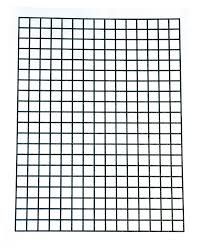
\includegraphics[angle = 90]{grid.jpg}}
2. Emily loves figuring out all the ways to arrange dominos. Help her find all the ways to arrange dominos in that are $2 \times 1$ in a $2 \times 1$,$2 \times 2$,$2 \times 3$ and $2 \times 4$ grid!\\\\\\\\
3. Now that you've helped Emily find how many ways to arrange the dominos in problem 2 she gets really philosophical. She starts pondering the nature of zero and wants you to help her find how many ways to arrange a $2 \times 1$ domino in a $2 \times 0$ grid. (You don't have to be too smart: Follow the pattern from problem 2)\\\\\\\\
4. We've had a lot of fun arranging dominos but now Emily wants a recursive formula for the ways to arrange $2 \times 1$ dominos. The key to finding recursive definitions is to find the answer to larger problems by finding the answer to smaller problems.\\\\
$D_n = $\# of tilings of a $2 \times n =$
\end{document}